%%RESULTADOS

\section{Evaluación de bloque de adquisición y decodificación}
Tras realizar la evaluación del subsistema de adquisición descrito en la sección \ref{Sec: Adquisicion} utilizando el procedimiento detallado en la sección \ref{Sec: EvalAdquisicion}, se obtuvo un valor de correlación promedio de 0.9615 $\pm$ 0.0604, el cual se obtuvo de un total de 27 registros realizados (3 repeticiones de cada una de las señales que conforman el banco de señales para evaluación de la adquisición). En la Figura \ref{Figura: ValProCum} se puede observar una comparación entre la señal patrón de 5 Hz y la señal adquirida con el subsistema diseñado en Simulink\textregistered. El Cuadro \ref{Cuadro:ValoresCorre} muestra el valor de correlación promedio obtenido para cada señal y la correlación total.

%Cuadro valores correlación
\begin{table}[htbp]
	\centering
	\begin{tabular}{|l|c|}
	\hline
	\textbf{} & \textbf{Correlación}\\ 
	\textbf{Señal} & \textbf{promedio}\\ \hline	\hline
	1 Hz & 0.9889\\ \hline
	5 Hz & 0.9428\\ \hline
	10 Hz & 0.9948\\ \hline
	20 Hz & 0.9933\\ \hline
	50 Hz & 0.9804\\ \hline
	100 Hz & 0.9334\\ \hline
	Atenuación lineal & 0.9466\\ \hline
	Atenuación exponencial & 0.8849\\ \hline
	Simulación contracción muscular & 0.9886\\ \hline
	\textbf{Correlación promedio total} & 0.9615\\ \hline
	\end{tabular}
	\caption{Valores de correlación promedio por señal y correlación promedio total.}
	\label{Cuadro:ValoresCorre}
\end{table}

%Senoidal obtenida tras para evaluación
\begin{figure}[htbp]
	\centering
	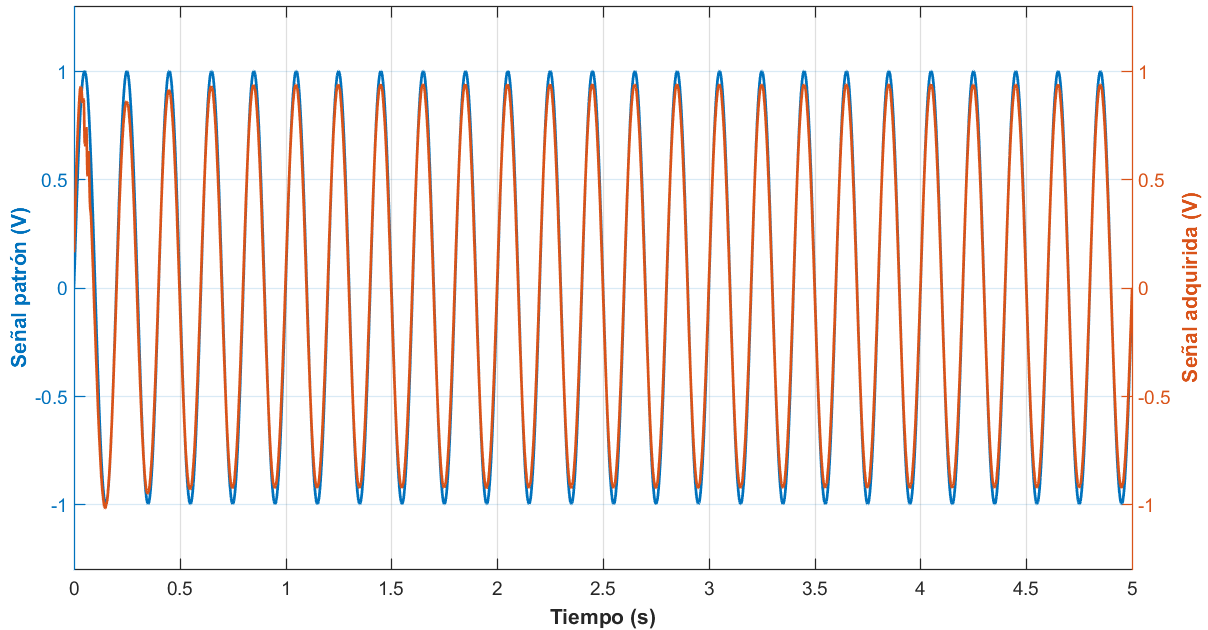
\includegraphics[width=\textwidth]{ValProCum.png}
	\caption[Comparación entre señales para evaluación de adquisición.]{Comparación entre señales para evaluación de adquisición. Señal patrón generada en MATLAB\textregistered \; (azul). Señal adquirida mediante el subsistema de adquisición diseñado en Simulink\textregistered \; (Rojo).}
	\label{Figura: ValProCum}
\end{figure}


\newpage
\section{Procesamiento de sEMG}
El esquema de filtrado utilizado (filtro pasa altas, filtro pasa bajas y filtro rechaza banda), al igual que el procesamiento para obtención del RMS suavizado, se pusieron a prueba fuera de línea con registros de sEMG de 10 voluntarios sanos (6 hombres y 4 mujeres en el rango de 20 a 24 años de edad).

La Figura \ref{Figura: Filtrado} muestra una comparación entre los canales de sEMG adquiridos para las pruebas de procesamiento y el resultado del filtrado fuera de línea. En la Figura \ref{Figura: RMS} se muestra un ejemplo del resultado del procesamiento para obtención de la envolvente RMS suavizada.

\begin{figure}[htbp]
	\centering
	\begin{subfigure}[htbp]{0.45\textwidth}
		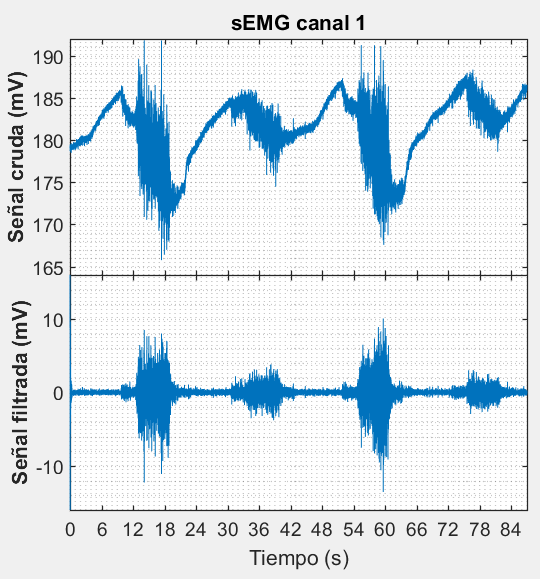
\includegraphics[width=\textwidth]{Filtrado_a.png}
		\caption{}
		\label{Figura: Filtrado_a}
	\end{subfigure}
	\hfill
	\begin{subfigure}[htbp]{0.45\textwidth}
		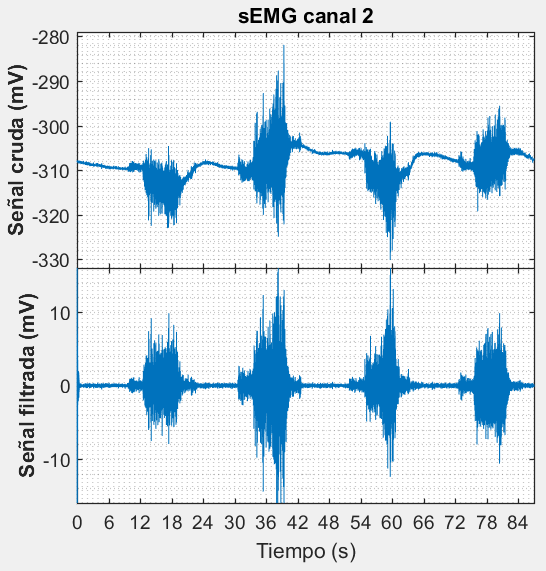
\includegraphics[width=\textwidth]{Filtrado_b.png}
		\caption{}
		\label{Figura: Filtrado_b}
	\end{subfigure}	
	\caption[Ejemplo representativo del funcionamiento del esquema de filtrado diseñado]{Ejemplo representativo del funcionamiento del esquema de filtrado diseñado.(a)Arriba, registro de sEMG del canal 1 sin filtrar.(a)Abajo, registro de sEMG del canal 1 después del filtrado.(b)Arriba, registro de sEMG del canal 2 sin filtrar.(b)Abajo, registro de sEMG del canal 2 después del filtrado.}
	\label{Figura: Filtrado}
\end{figure}

\begin{figure}[htbp]
	\centering
	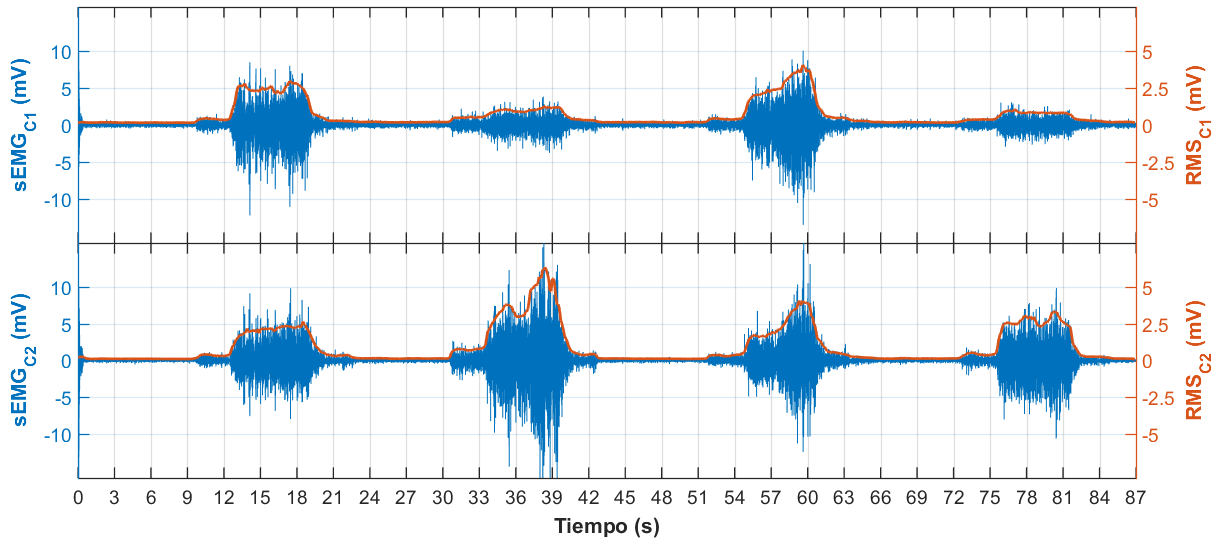
\includegraphics[width=\textwidth]{RMS.png}
	\caption[Ejemplo representativo de la obtención de envolvente de RMS]{Ejemplo representativo de la obtención de envolvente de RMS. En azul, los registros de sEMG después del filtrado. En rojo, las envolventes de RMS. Arriba, señal sEMG y envolvente del canal 1, correspondiente al movimiento de pinza gruesa. Abajo, señal sEMG y envolvente del canal 2, correspondiente al movimiento de apertura de mano.}
	\label{Figura: RMS}
\end{figure}


\newpage
\section{Sistema de control}
El sistema de control sEMG-FES se puso a prueba con un voluntario sano de 22 años de edad, obteniendo los siguientes resultados.

\subsection{Calibración}
Tras realizar el proceso de calibración descrito en la sección \ref{Sec: Calibracion} se obtuvieron los valores mostrados en los Cuadros \ref{Cuadro:UmbralesFES} a \ref{Cuadro:Rectas}.

El Cuadro \ref{Cuadro:UmbralesFES} muestra los valores obtenidos para los umbrales motores y funcionales tras realizar la calibración de parámetros FES descrita en la sección \ref{Sec:CalFES}.

El Cuadro \ref{Cuadro:UmbralesRMS} muestra los valores de umbrales RMS y el valor del umbral detector de movimiento obtenidos tras realizar la calibración de umbrales RMS de sEMG descrita en la sección \ref{Sec:CalRMS}. Cabe señalar que en esta prueba se obtuvo un umbral de activación menor para el movimiento de pinza gruesa en comparación con el umbral de activación para el movimiento de apertura de mano (recordemos que los umbrales de activación son el umbral de pinza gruesa incompleta en el canal 1 y el umbral de apertura de mano incompleta en el canal 2).

El Cuadro \ref{Cuadro:Rectas} muestra los valores de la pendiente y la ordenada al origen correspondientes a las rectas de mapeo proporcional para el canal 1 y el canal 2 de estimulación eléctrica.

%Cuadro umbrales FES
\begin{table}[htbp]
	\centering
	\begin{tabular}{|l|c|c|}
	\hline
	\textbf{} & \textbf{Umbral motor} & \textbf{Umbral funcional}\\
	\textbf{} & \textbf{($U_{Mj}$)} & \textbf{($U_{Fj}$)}\\
	\textbf{Canal} & \textbf{[mA]} & \textbf{[mA]}\\ \hline	\hline
	Canal 1 (Pinza gruesa) & 6 & 14\\ \hline
	Canal 1 (Apertura de mano) & 9 & 13\\ \hline
	\end{tabular}
	\caption{Valores obtenidos para umbrales motores y funcionales de estimulación eléctrica.}
	\label{Cuadro:UmbralesFES}
\end{table}

%Cuadro umbrales sEMG
\begin{table}[htbp]
	\centering
	\begin{tabular}{|l|c|c|}
	\hline
	\textbf{} & \multicolumn{2}{|c|}{Umbral RMS}\\
	\textbf{} & \textbf{Canal 1} & \textbf{Canal 2}\\
	\textbf{} & \textbf{$j=1$} & \textbf{$j=2$}\\
	\textbf{Movimiento} & \textbf{[mV]} & \textbf{[mV]}\\ \hline \hline
	Apertura de mano completa ($M_{1j}$) & 0.8708 & 3.0000\\ \hline
	Apertura de mano incompleta	($M_{2j}$) & 0.4657 & 0.9115\\ \hline
	Descanso ($M_{3j}$) & 0.1981 & 0.1536\\ \hline
	Pinza gruesa incompleta ($M_4j$) & 0.7918 & 0.8134\\ \hline
	Pinza gruesa completa ($M_5j$) & 2.2491 & 1.9610\\ \hline	
	Umbral detector de movimiento ($UDM$) & \multicolumn{2}{|c|}{0.4458}\\ \hline
	\end{tabular}
	\caption{Valores obtenidos para umbrales RMS de sEMG.}
	\label{Cuadro:UmbralesRMS}
\end{table}

%Cuadro parámetros de rectas
\begin{table}[htbp]
	\centering
	\begin{tabular}{|l|c|c|}
	\hline
	\textbf{} & \textbf{Pendiente} & \textbf{Ordenada al origen}\\ 
	\textbf{} & \textbf{($m_{j}$)} & \textbf{($b_{j}$)}\\
	\textbf{Canal} & \textbf{[mA/mV]} & \textbf{[mA]}\\\hline \hline
	Canal 1 (Pinza gruesa) & 5.4894 & 1.6536\\ \hline
	Canal 2 (Apertura de mano) & 1.9153 & 7.2542\\ \hline
	\end{tabular}
	\caption{Parámetros de recta obtenidos para realizar mapeo sEMG-FES.}
	\label{Cuadro:Rectas}
\end{table}


\newpage
\subsection{Validación fuera de línea}
El algoritmo de clasificación de movimientos obtuvo una exactitud del 81.7241\%, valor derivado de la matriz de confusión mostrada en el Cuadro \ref{Cuadro:PorcentajesValores}. La Figura \ref{Figura: MapOff} muestra el resultado de la prueba para la validación fuera de línea, donde se pueden observar los siguientes resultados de clasificación:

\begin{itemize}
	\item Durante los episodios del movimiento de cierre de mano (9-21 y 51-63 s):
	
	\begin{itemize}
		\item Se puede observar una clasificación correcta cuando la señal \emph{Acción} toma como valores a \emph{CI} y \emph{CC} y la señal \emph{Amplitud FES$_{C1}$} toma valores distintos de cero mientras que la señal \emph{Amplitud FES$_{C2}$} toma valor de cero.
		\item Dentro de los episodios de este movimiento se pueden observar errores de clasificación en los segundos 18-21 y alrededor de los 59 segundos, donde se observa que la señal \emph{Amplitud FES$_{C2}$} toma valores distintos de cero.
	\end{itemize}
	
	\item Durante los episodios del movimiento de apertura de mano (30-42 y 72-84 s):
	
	\begin{itemize}
		\item Se puede observar una clasificación correcta cuando la señal \emph{Acción} toma como valores a \emph{AI} y \emph{AC} y la señal \emph{Amplitud FES$_{C2}$} toma valores distintos de cero mientras que la señal \emph{Amplitud FES$_{C1}$} toma valor de cero.
		\item Dentro de los episodios de este movimiento se pueden observar errores de clasificación en los segundos 30-33, 40-42 y 72-75, donde se observa que la señal \emph{Amplitud FES$_{C1}$} toma valores distintos de cero.
	\end{itemize}
		
	\item Durante los episodios de descanso (0-9, 21-30, 42-51, 63-72 y 84-87 s):
	\begin{itemize}
		\item Se puede observar una clasificación correcta cuando la señal \emph{Acción} toma como valor a \emph{DD} y las señales \emph{Amplitud FES$_{C1}$} y \emph{Amplitud FES$_{C2}$} toman valor de cero.
		\item Dentro de los episodios de este movimiento se pueden observar errores alrededor de los segundos 42 y 63, donde la señal \emph{Amplitud FES$_{C1}$} se activa brevemente cuando no tendría que haberse activado.
	\end{itemize}
\end{itemize}

%Cuadro porcentajes aciertos y errores 
\begin{table}[htbp]
	\centering
\begin{tabular}{|l|c|c|c|}
	\hline
	\textbf{} & \multicolumn{3}{|c|}{Movimiento real}\\
	\textbf{Movimiento} & \textbf{Descanso} & \textbf{Pinza} & \textbf{Apertura}\\
	\textbf{predicho} & \textbf{} & \textbf{gruesa} & \textbf{de mano}\\ \hline \hline
	\textbf{Descanso} & \textbf{381} & \textbf{9} & \textbf{0}\\ \hline
	\textbf{Pinza gruesa} & \textbf{41} & \textbf{192} & \textbf{7}\\ \hline
	\textbf{Apertura de mano} & \textbf{32} & \textbf{70} & \textbf{138}\\ \hline
	\end{tabular}
	\caption{Matriz de confusión obtenida tras validación fuera de línea.}
	\label{Cuadro:PorcentajesValores}
\end{table}

%Figura validación fuera de línea
\begin{figure}[htbp]
	\centering
	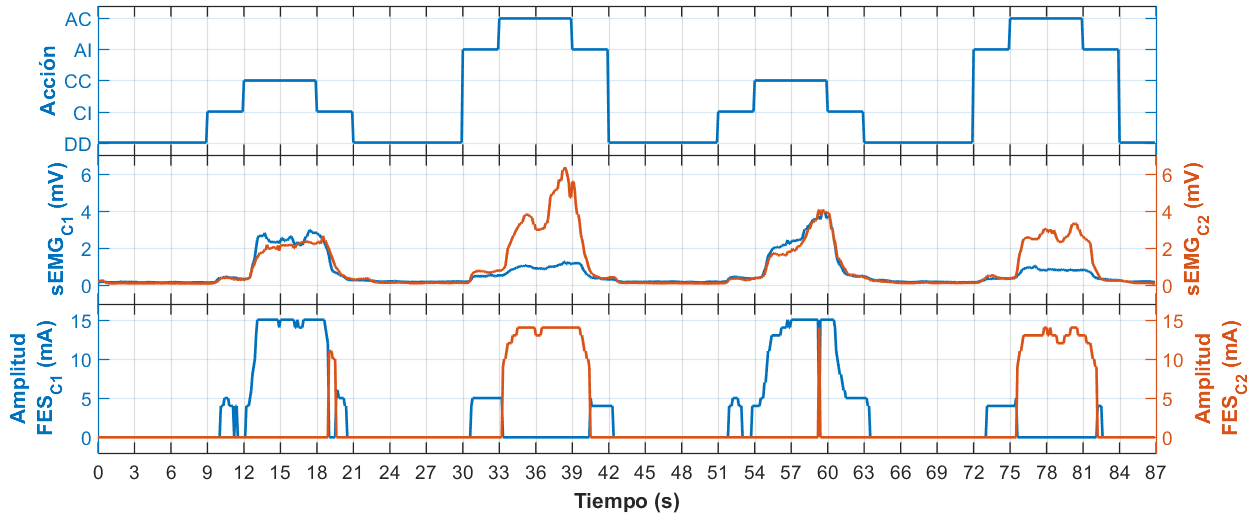
\includegraphics[width=\textwidth]{MapOff.png}
	\caption[Secuencia temporal de una prueba exitosa de validación fuera de línea]{Secuencia temporal de una prueba exitosa de validación fura de línea del sistema de control sEMG-FES. Arriba: Marcadores de acción solicitada al sujeto (descanso (DD), pinza gruesa incompleta (CI), pinza gruesa completa (CC), apertura de mano incompleta (AL), apertura de mano completa (AC)). Centro: Envolventes de sEMG (Azul: canal 1. Rojo: canal 2). Abajo: Amplitudes de estimulación eléctrica (salida del sistema de control) (Azul: canal 1. Rojo: canal 2). }
	\label{Figura: MapOff}
\end{figure}


\newpage
\subsection{Validación en línea (control por biofeedback)}
Respecto a la prueba de validación en línea, en esta demostró una respuesta del sistema de acuerdo a lo esperado. La Figura \ref{Figura: MapOn} presenta un segmento de las señales obtenidas tras la realización de la prueba en línea.

%Figura prueba en línea (sin estimulación)
\begin{figure}[htbp]
	\centering
	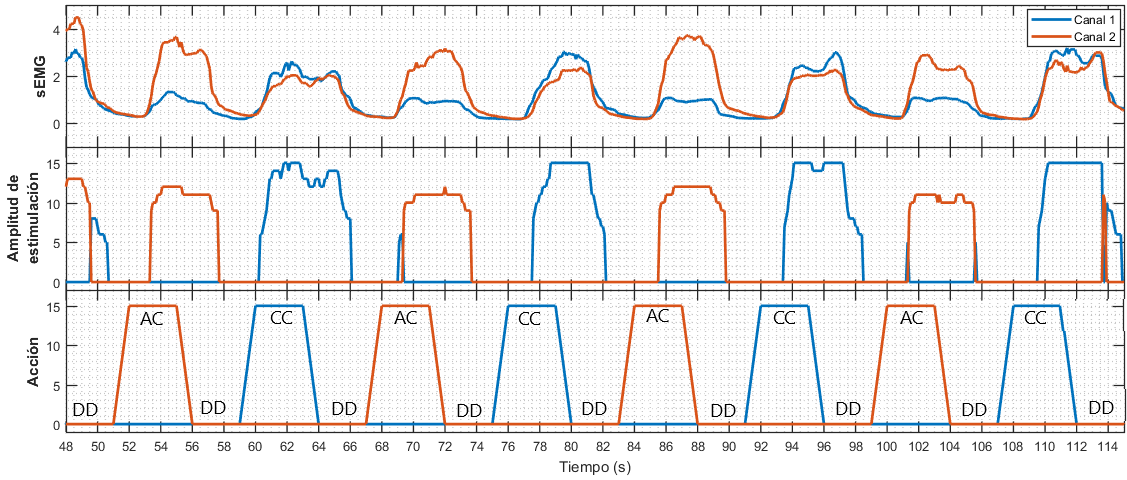
\includegraphics[width=\textwidth]{MapOn.png}
	\caption[Secuencia temporal de una prueba exitosa de validación en línea]{Secuencia temporal de una prueba exitosa de validación en línea del sistema de control sEMG-FES.  Arriba: Señal trapezoidal patrón indicadora del movimiento objetivo (descanso (DD), pinza gruesa (CC), apertura de mano completa (AC)). Centro: Envolventes de sEMG (Azul: canal 1. Rojo: canal 2). Abajo: Amplitudes de estimulación eléctrica (salida del sistema de control) (Azul: canal 1. Rojo: canal 2).}
	\label{Figura: MapOn}
\end{figure}


\subsection{Validación en línea con FES}
En relación a la validación en línea con FES, el sistema logró llevar a cabo la modulación de la estimulación eléctrica de forma satisfactoria, obteniendo un retardo promedio del sistema con valor de de 2.3 $\pm$ 0.3553 s, medido de la forma descrita en la sección \ref{Sec: TareaObj}. La Figura \ref{Figura: Retardo} muestra un acercamiento a las señales obtenidas al termino de la prueba de la validación en línea con FES, donde se aprecia el retardo entre la señal patrón y la señal de amplitud de estimulación eléctrica.

\newpage
%Figura medición de retardo
\begin{figure}[htbp]
	\centering
	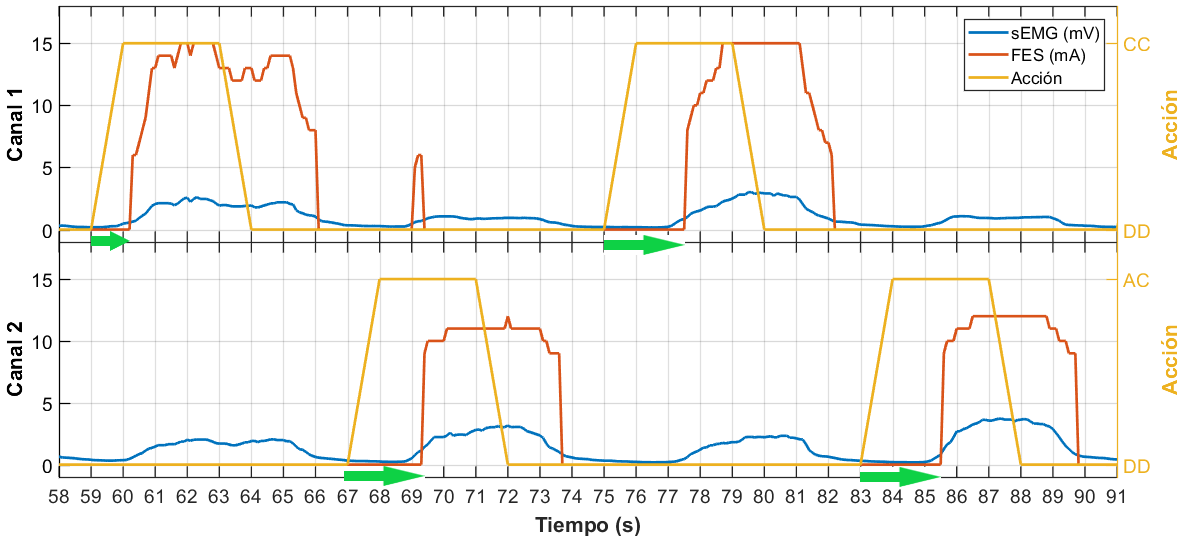
\includegraphics[width=\textwidth]{Retardo_Flechas_2.png}
	\caption[Secuencia temporal de una prueba exitosa de la validación en línea con FES]{Secuencia temporal de una prueba exitosa de la validación en línea con FES. Se muestran las diferentes señales asociadas a cada movimiento sobre la misma base de tiempo para visualizar el retardo existente entre la señal trapezoidal patrón y la señal de amplitud de estimulación eléctrica. Arriba: Señales para movimiento pinza gruesa completa (CC). Abajo: Señales para movimiento apertura de mano completa (AC). En amarillo se muestra la señal trapezoidal patrón del movimiento objetivo. En azul se muestra la envolvente de sEMG. En rojo se muestra la amplitud de estimulación eléctrica (salida del sistema control). Se agregaron flechas color verde a las gráficas para resaltar el retardo existente entre la señal trapezoidal y la amplitud FES. La escala vertical mostrada a la izquierda es la misma para las señales sEMG y FES, sólo se aplica el correspondiente cambio de unidades.}
	\label{Figura: Retardo}
\end{figure}


\subsection{Tarea funcional asíncrona}
Respecto a la tarea funcional asíncrona, esta logró ser realizada por el sujeto de prueba, logrando realizar las 6 acciones de la que consta dicha tarea. La Figura \ref{Figura: TareaFuncional} muestra las diferentes fases de movimiento durante la ejecución de la tarea funcional asíncrona por parte del sujeto, mientras que la Figura \ref{Figura: TareaFuncional_Senales} muestra las señales (sEMG y FES) correspondiente a cada fase. Se puede apreciar que los movimientos corresponden a los descritos en la sección \ref{Sec: TareaFunAsin}.

%Figura levantar objetos
\begin{figure}[htbp]
	\centering
	\begin{subfigure}[htbp]{0.45\textwidth}
		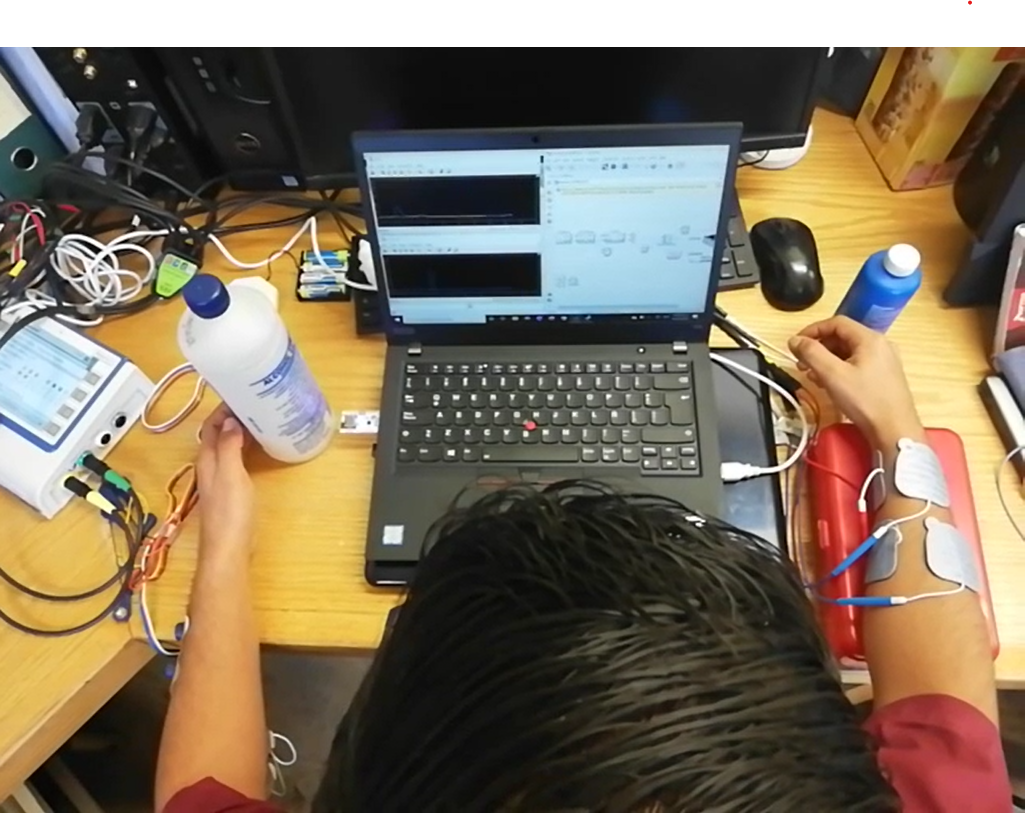
\includegraphics[width=\textwidth]{Funcional_a.png}
		\caption{}
		\label{Figura: Fun_A}
	\end{subfigure}
	\begin{subfigure}[htbp]{0.45\textwidth}
		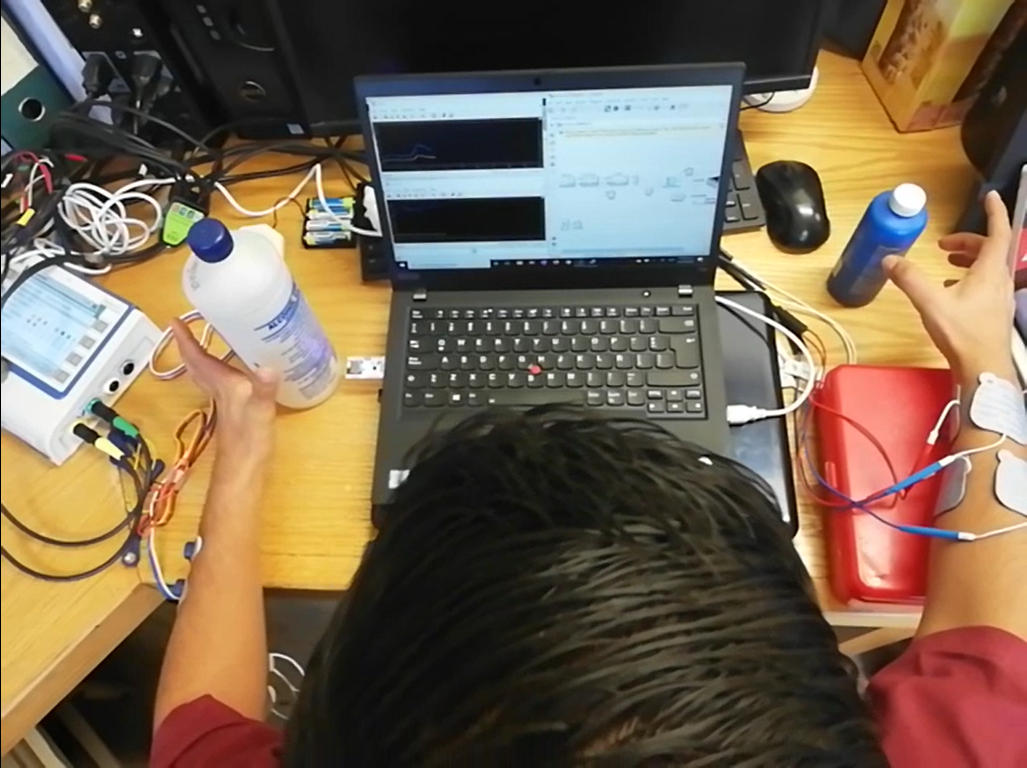
\includegraphics[width=\textwidth]{Funcional_b.png}
		\caption{}
		\label{Figura: Fun_B}
	\end{subfigure}
	\newline
	\begin{subfigure}[htbp]{0.45\textwidth}
		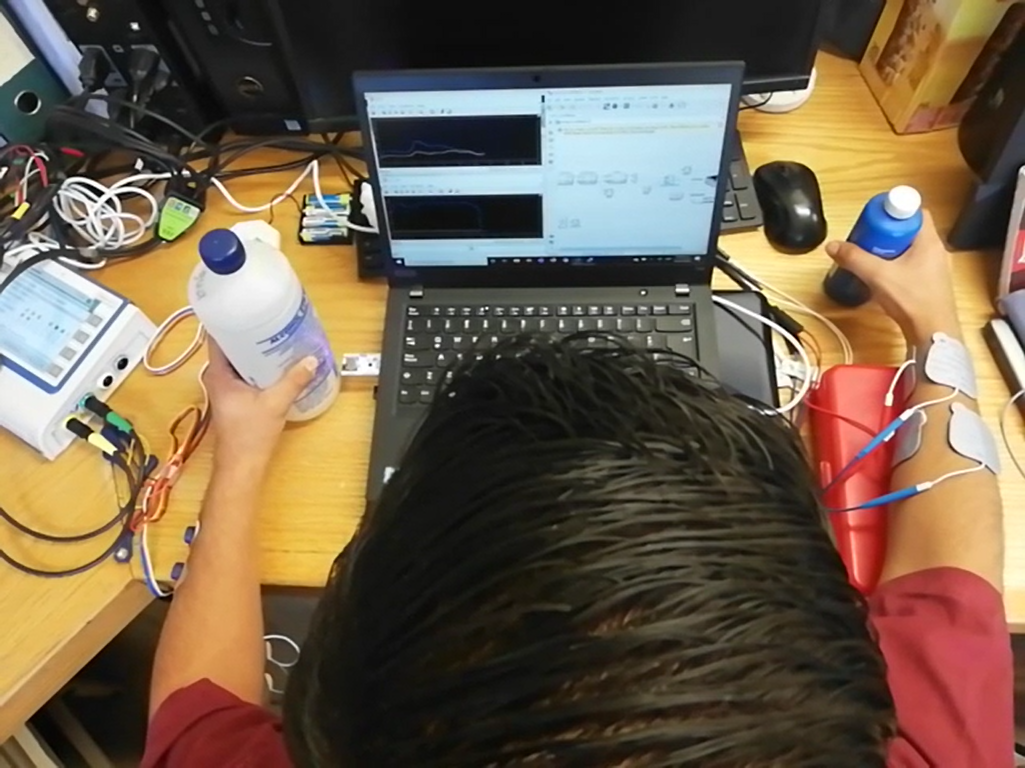
\includegraphics[width=\textwidth]{Funcional_c.png}
		\caption{}
		\label{Figura: Fun_C}
	\end{subfigure}
	\begin{subfigure}[htbp]{0.45\textwidth}
		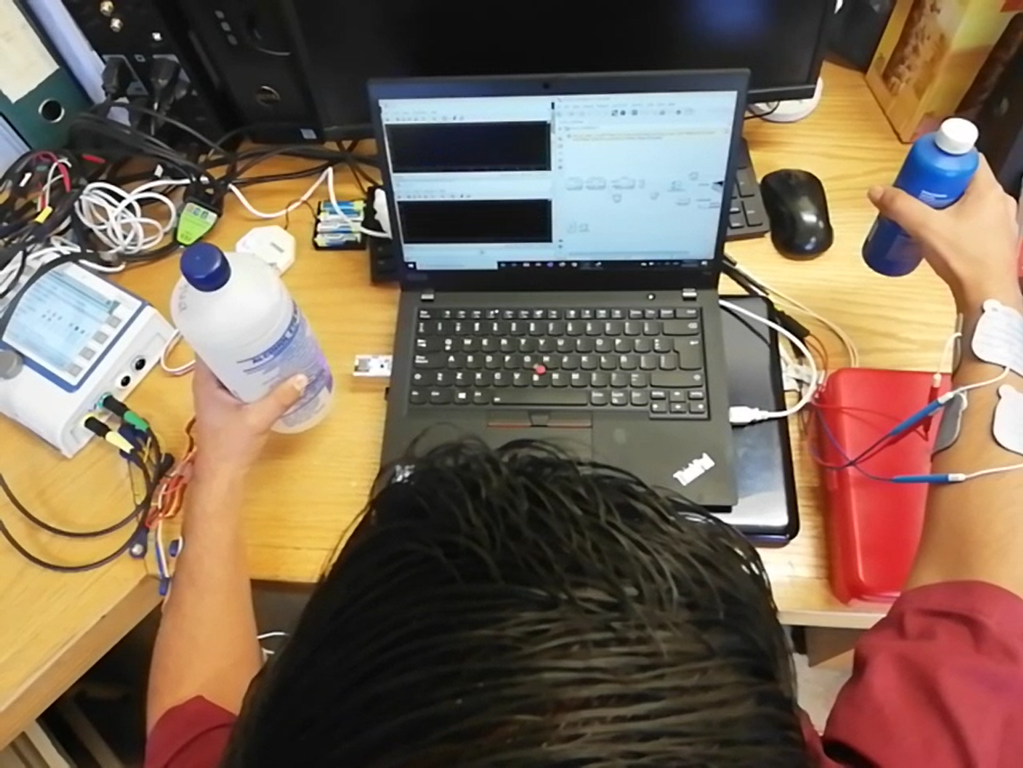
\includegraphics[width=\textwidth]{Funcional_d.png}
		\caption{}
		\label{Figura: Fun_D}
	\end{subfigure}
	\newline
	\begin{subfigure}[htbp]{0.45\textwidth}
		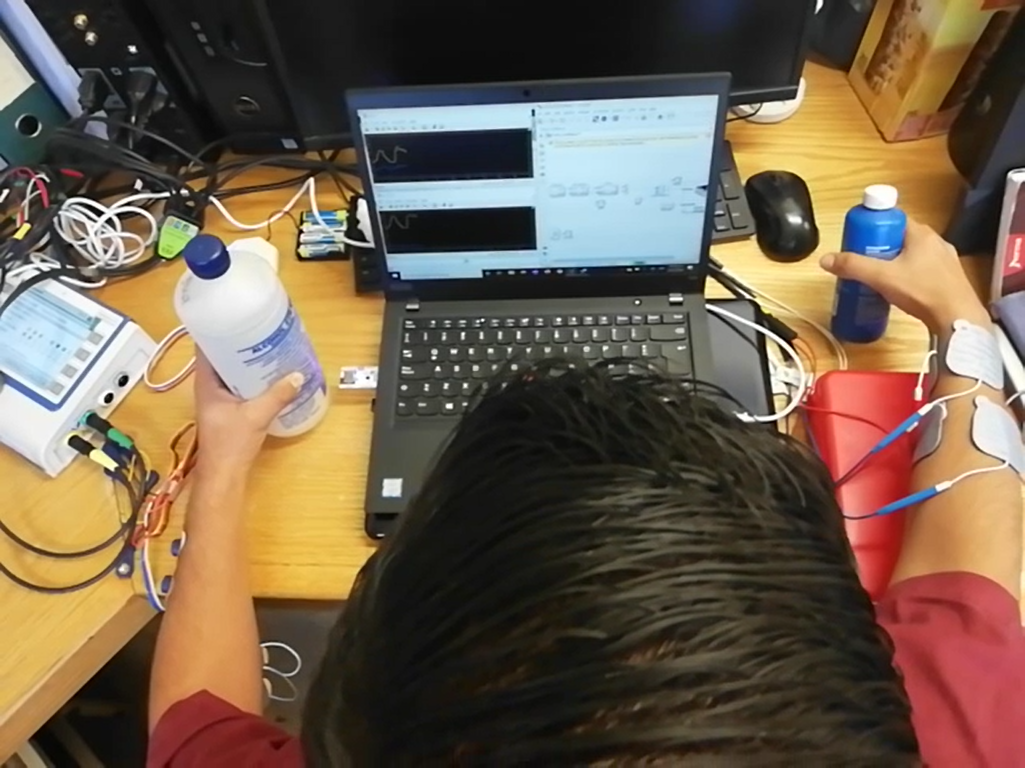
\includegraphics[width=\textwidth]{Funcional_e.png}
		\caption{}
		\label{Figura: Fun_E}
	\end{subfigure}
	\begin{subfigure}[htbp]{0.45\textwidth}
		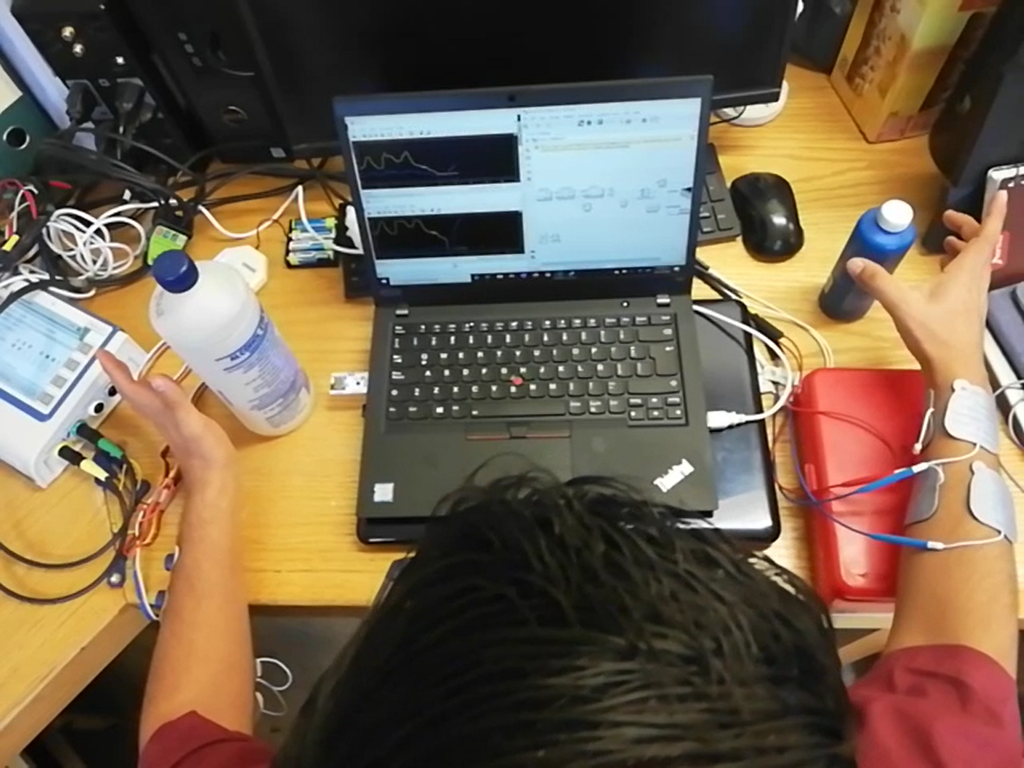
\includegraphics[width=\textwidth]{Funcional_f.png}
		\caption{}
		\label{Figura: Fun_F}
	\end{subfigure}
	\caption[Fases de la tarea funcional asíncrona ejecutada por el sujeto (en línea)]{Fases de la tarea funcional asíncrona ejecutada por el sujeto (en línea). (a)Adducción de hombros. (b)Extensión de dedos. (c)Flexión de dedos. (d)Abducción y extensión de hombros. (e)Flexión de hombros. (f) Extensión de dedos.}
	\label{Figura: TareaFuncional}
\end{figure}

%Figura señales levantar objetos
\begin{figure}[htbp]
	\centering
	\begin{subfigure}[htbp]{0.35\textwidth}
		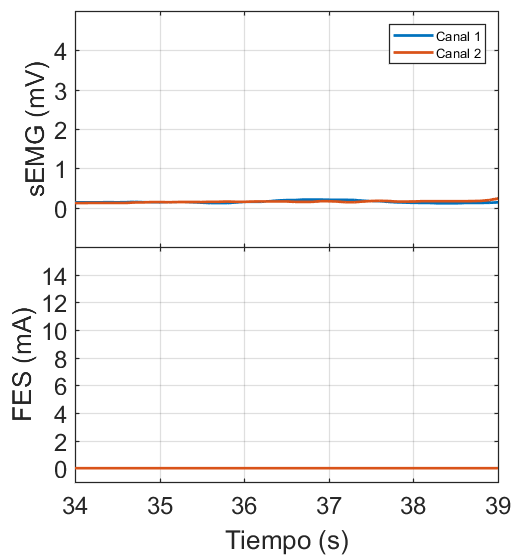
\includegraphics[width=\textwidth]{sEMG_FES_FUN_a.png}
		\caption{}
		\label{Figura: Fun_Sen_A}
	\end{subfigure}
	\hspace*{1cm}
	\begin{subfigure}[htbp]{0.35\textwidth}
		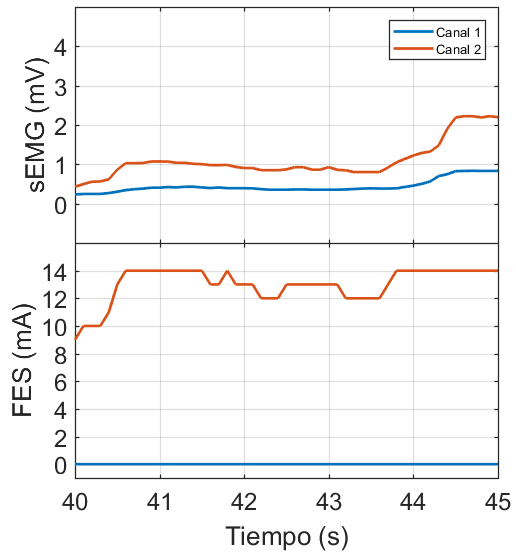
\includegraphics[width=\textwidth]{sEMG_FES_FUN_b.png}
		\caption{}
		\label{Figura: Fun_Sen_B}
	\end{subfigure}
	\newline
	\begin{subfigure}[htbp]{0.35\textwidth}
		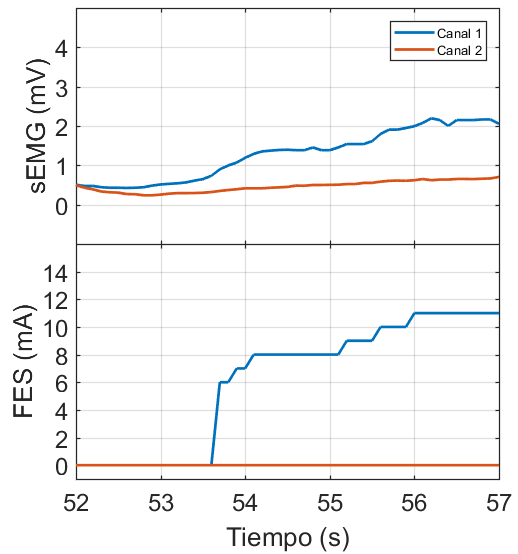
\includegraphics[width=\textwidth]{sEMG_FES_FUN_c.png}
		\caption{}
		\label{Figura: Fun_Sen_C}
	\end{subfigure}
	\hspace*{1cm}
	\begin{subfigure}[htbp]{0.35\textwidth}
		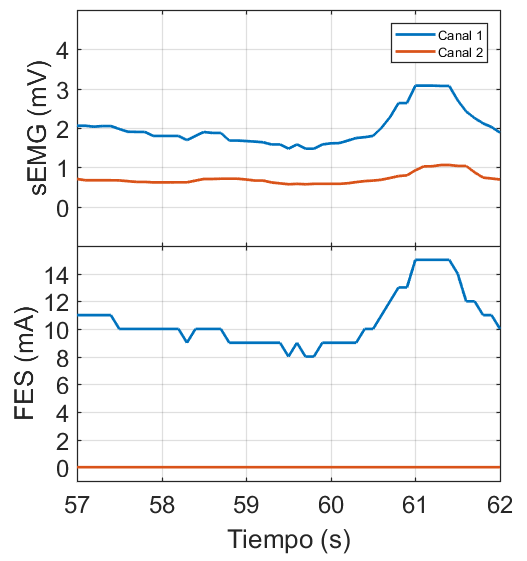
\includegraphics[width=\textwidth]{sEMG_FES_FUN_d.png}
		\caption{}
		\label{Figura: Fun_Sen_D}
	\end{subfigure}
	\newline
	\begin{subfigure}[htbp]{0.35\textwidth}
		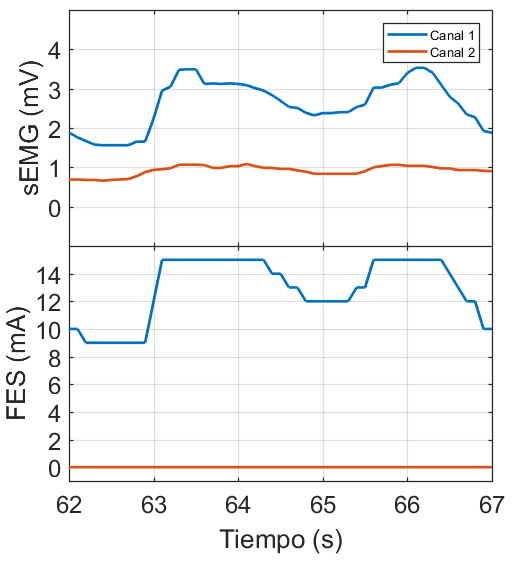
\includegraphics[width=\textwidth]{sEMG_FES_FUN_e.png}
		\caption{}
		\label{Figura: Fun_Sen_E}
	\end{subfigure}
	\hspace*{1cm}
	\begin{subfigure}[htbp]{0.35\textwidth}
		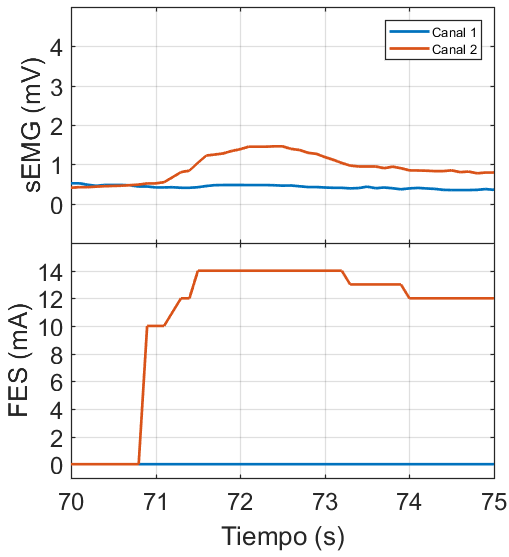
\includegraphics[width=\textwidth]{sEMG_FES_FUN_f.png}
		\caption{}
		\label{Figura: Fun_F}
	\end{subfigure}
	\caption[Señales de las fases de la tarea funcional asíncrona ejecutada por el sujeto (en línea)]{Señales de las fases de la tarea funcional asíncrona ejecutada por el sujeto (en línea). Arriba: Señales de sEMG. Abajo: Señales de amplitud FES. Azul: Señales del canal 1. Rojo: Señales del canal 2. (a)Adducción de hombros. (b)Extensión de dedos. (c)Flexión de dedos. (d)Abducción y extensión de hombros. (e)Flexión de hombros. (f) Extensión de dedos.}
	\label{Figura: TareaFuncional_Senales}
\end{figure}
